\documentclass[letter]{article}
\usepackage{amsmath}
\usepackage{amssymb}
\usepackage{graphicx}

\setlength\oddsidemargin{0.25in}
\setlength\evensidemargin{0.25in}
\setlength\topmargin{0.0in}
\setlength\textheight{8in}
\setlength\textwidth{6in}
\setlength\parindent{0in}

\usepackage{fancyhdr}
\pagestyle{fancy}

\fancyhead[L]{Transformations of the plane}
\fancyhead[C]{Tech 411.05 {\em Patterns and Symmetry}}
\fancyhead[R]{\thepage}
\fancyfoot{}

\newcommand{\bx}{{\bf x}}

\begin{document}

A figure in a plane can move in several ways without changing its shape.
\begin{itemize}
\item {\bf rotation:} changing the tilt of the shape with respect to the coordinate axes
\item {\bf reflection:} picking up the shape, flipping it over, and placing it back down
\item {\bf translation:} shifting left/right or up/down with no change of orientation
\end{itemize}
With this worksheet you will develop mathematical representations of these transformations
using geometry, algebra, vectors, and matrices.

\section{Rotations}

\begin{center}
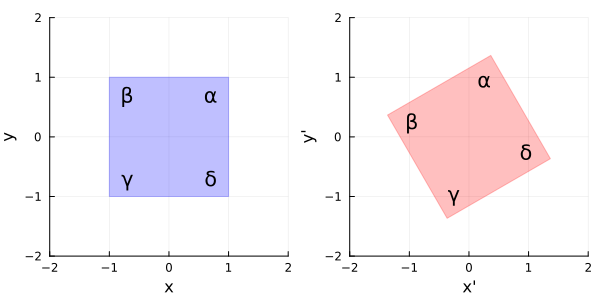
\includegraphics[width=0.75\textwidth]{rotation_square.png}
\end{center}
The figure above shows the rotation of a square by $\pi/6$ (or $30^\circ$).
We use $(x,y)$ coordinates for the original square on the left and $(x',y')$
coordinates for the rotated square on the right. Each point $(x,y)$ in the
original square moves to a point $(x', y')$ in the rotated square according to
equations of form
\begin{align}
  x' &= ax + by \\
  y' &= cx + dy \nonumber
\end{align}
where $a,b,c,$ and $d$ are constants determined by the rotation angle. 

\vspace{2mm}
{\bf Problem 1:} Figure out the values of $a,b,c,$ and $d$ as functions
of the rotation angle $\theta$. 

\vspace{2mm}
{\bf Strategy:} There are four unknowns $a,b,c,d$, so we need four equations to solve for them.
Choose a point on the original square, say vertex $\alpha$ at $(x,y) = (1,1)$. Use trigonometry
to find the position $(x',y')$ of vertex $\alpha$ after rotation as a function of the rotation angle
$\theta$. Then plug those values of $(x,y)$ and $(x',y')$ into the above equations. That gives
you two equations. Do the same for another point, say vertex $\beta$, to get two more equations.
Solve the four equations to get $a,b,c,d$ as trigonometric functions of $\theta$.

\newpage

\vspace{2mm}
{\bf Hint:} If you use the points $(x,y) = (0,1)$ and $(x,y) = (1,0)$ instead of the
vertices $\alpha$ and $\beta$, the trigonometry and algebra are much simpler.

\begin{center}
  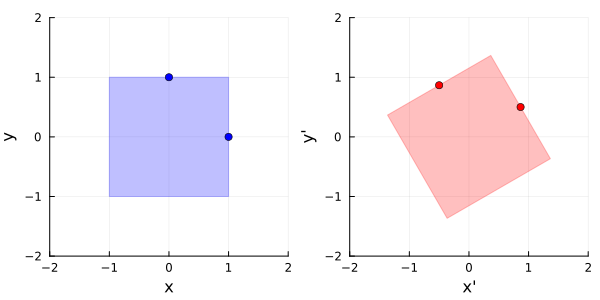
\includegraphics[width=0.75\textwidth]{rotation_square_b.png}
\end{center}

\newpage

{\bf Problem 2:} Rewrite your answer to problem 1 as a matrix-vector multiplication.

\vspace{2mm}
{\bf Guidance:} The equations 
\begin{align}
  x' &= ax + by \nonumber \\      
  y' &= cx + dy         \label{linreln_algebra}
\end{align}
can be written as a matrix-vector multiplication 
\begin{align}
  \begin{bmatrix} x' \\ y' \end{bmatrix}
  =
  \begin{bmatrix} a & b \\ c & d \end{bmatrix}                       
  \begin{bmatrix} x \\ y \end{bmatrix}.  \label{linreln_matrix}
\end{align}
This is just a graphical way to represent the original equations.

\vspace{3mm}
$\begin{bmatrix} x' \\ y' \end{bmatrix}$ and $\begin{bmatrix} x \\ y \end{bmatrix}$
are {\em vectors} representing the coordinates $(x',y')$ and $(x,y)$ as points on a plane.

\vspace{3mm}
$\begin{bmatrix} a & b \\ c & d \end{bmatrix}$ is a {\em matrix} that specifies
the functional relationship between the vectors $(x',y')$ and $(x,y)$.

\vspace{3mm}
Matrix-vector multiplication is defined by the ``across and down'' rule. For example,
the product 
\begin{align*}
  \begin{bmatrix} 2 & 1 \\ 3 & -4 \end{bmatrix}                       
  \begin{bmatrix} 5 \\ 6 \end{bmatrix} 
\end{align*}
is found by multiplying each entry {\em across} the first row of the matrix by the entries
going {\em down} the vector and adding,
\begin{align*}
  \begin{bmatrix} 2 & 1 \\  & \end{bmatrix}
  \begin{bmatrix} 5 \\ 6 \end{bmatrix}  \quad
  =
  \begin{bmatrix} 2 \cdot 5 + 1 \cdot 6 \\ \phantom{5} \end{bmatrix} 
  = 
  \begin{bmatrix} 16 \\  \phantom{5} \end{bmatrix},
\end{align*}
and then doing the same going across the bottom row of the matrix to get
\begin{align*}
  \begin{bmatrix}  \\  3 & -4 \end{bmatrix}
  \begin{bmatrix} 5 \\ 6 \end{bmatrix} \quad
  =
  \begin{bmatrix} \phantom{5} \\ 3 \cdot 5 - 4 \cdot 6 \end{bmatrix} 
  = 
  \begin{bmatrix} \phantom{16} \\  -9 \end{bmatrix}.
\end{align*}
Thus
\begin{align*}
  \begin{bmatrix} 2 & 1 \\ 3 & -4 \end{bmatrix}                       
  \begin{bmatrix} 5 \\ 6 \end{bmatrix}
  =
  \begin{bmatrix} 16 \\ -9\end{bmatrix}.                       
\end{align*}

Similarly, 
\begin{align}
  \begin{bmatrix} x' \\ y' \end{bmatrix}
  =
  \begin{bmatrix} a & b \\ c & d \end{bmatrix}                       
  \begin{bmatrix} x \\ y \end{bmatrix}
  =
  \begin{bmatrix} ax + by \\ cx + dy \end{bmatrix}.
\end{align}
This is just equation \ref{linreln_algebra} written as an equality of two vectors.
So to get your answer for problem 2, just substitute the trigonometric functions
for $a,b,c,d$ that you derived in problem 1 into equation \ref{linreln_matrix}.



\section{Reflections}

{\bf Problem 3:} Using similar methods as in problems 1 and 2, derive a matrix-vector
representation of reflection about the vertical axis. 

\begin{center}
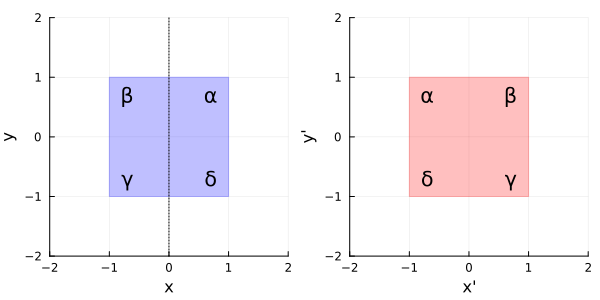
\includegraphics[width=0.75\textwidth]{xreflection.png}
\end{center}

Your answer will be of the form $
  \begin{bmatrix} x' \\ y' \end{bmatrix}
  =
  \begin{bmatrix} a & b \\ c & d \end{bmatrix}                       
  \begin{bmatrix} x \\ y \end{bmatrix}
$
with specific numeric values for $a,b,c,d$.

\newpage

{\bf Problem 4:} Do the same as problem 3 for reflection about the horizontal axis. 

\begin{center}
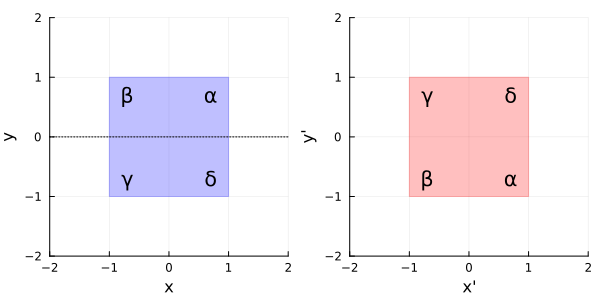
\includegraphics[width=0.75\textwidth]{yreflection.png}
\end{center}

\newpage

{\bf Problem 5 (challenge):} Derive a matrix-vector representation of a reflection
about a diagonal line at angle $\pi/4$ ($45^\circ$). 

\begin{center}
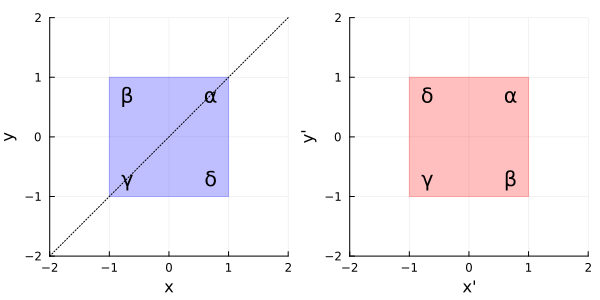
\includegraphics[width=0.75\textwidth]{diagonalreflection.png}
\end{center}
\newpage

\section{Chained transformations, matrix-matrix multiplication.}


Here we see a rotation of a square by $\theta = \pi/6$ followed by a reflection
about the vertical axis.

\begin{center}
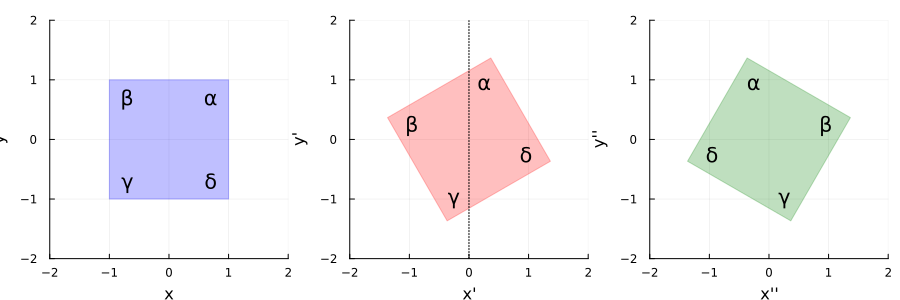
\includegraphics[width=\textwidth]{chained-transformation-1.png}
\end{center}

\vspace{4mm}
{\bf Problem 6 (challenge):} Express the chained transformation from $\bx$ to $\bx''$
as a matrix-vector multiplication. 

\vspace{4mm}
{\bf Strategy:}
You should have the reflection as a matrix-vector product from problem 3,
and you can get the rotation matrix by plugging in $\theta = \pi/6$ to your
answer for problem 1.

\vspace{4mm}
Let the rotation and reflection matrices and the coordinate vector $(x,y)$ be labeled
as follows
\begin{align*}
  R = \begin{bmatrix} r_{11} & r_{12} \\ r_{21} & r_{22} \end{bmatrix}, \quad \quad
  S = \begin{bmatrix} s_{11} & s_{12} \\ s_{21} & s_{22} \end{bmatrix}, \quad \quad
  \bx = \begin{bmatrix} x \\ y \end{bmatrix}.                                                                                                
\end{align*}
Your $R$ and $S$ matrices will have specific numerical values instead of symbols, but I'll
use symbols as above to avoid giving away the answers for previous problems! 
  
\vspace{4mm}
Then the rotation transformation is $\bx' = R \bx$, and the reflection is $\bx'' = S \bx'$,
and the chained transformation is $\bx'' = S \bx' = S(Rx)$. Writing that out in long-hand form,

\begin{align}
  \begin{bmatrix} x'' \\ y'' \end{bmatrix}
                        =
  \begin{bmatrix} s_{11} & s_{12} \\ s_{21} & s_{22} \end{bmatrix}
  \left(\begin{bmatrix} r_{11} & r_{12} \\ r_{21} & r_{22} \end{bmatrix}
  \begin{bmatrix} x \\ y \end{bmatrix} \right) \label{SRx}
\end{align}
Again, you will have specific numebrs for the matrix coefficients instead of symbols.

\vspace{4mm}
Now do across-and-down on the $Rx$ multiplication to get $Rx$ expressed as a vector.
Then do across-and-down on the $S (Rx)$ multiplication. You should end up with a vector
whose components are sums of $x$ and $y$ times some numeric coefficients. Then rewrite
that vector as a single matrix-vector multiplication, where the coefficients go in the matrix,
and the vector is $\bx = \begin{bmatrix} x \\ y \end{bmatrix}$. The answer should look like
\begin{align}
  \begin{bmatrix} x'' \\ y'' \end{bmatrix}
                        =
  \begin{bmatrix} ? & ? \\ ? & ? \end{bmatrix}
  \begin{bmatrix} x \\ y \end{bmatrix} \label{answerform}
\end{align} 
with specific numbers in place of the question marks.
\newpage

\vspace{4mm}
{\bf Problem 7 (challenge):} Do the same as in problem 6, but using symbols rather than
specific numbers for the matrices. Start directly from equation \ref{SRx}, and end up
with something like equation \ref{answerform}. But instead of numbers for the matrix elements,
you will have expressions involving $r_{11},$ $r_{12}$, $\ldots$ and $s_{11},$ $s_{12}$, $\ldots$.


\vspace{180mm}
{\bf A question to ponder:} Why do mirrors reverse images left to right, but not upside down?

\end{document}
